\documentclass[border=10pt]{standalone}
\usepackage{tikz}
\usetikzlibrary{arrows.meta}
\usepackage{xcolor}

\begin{document}

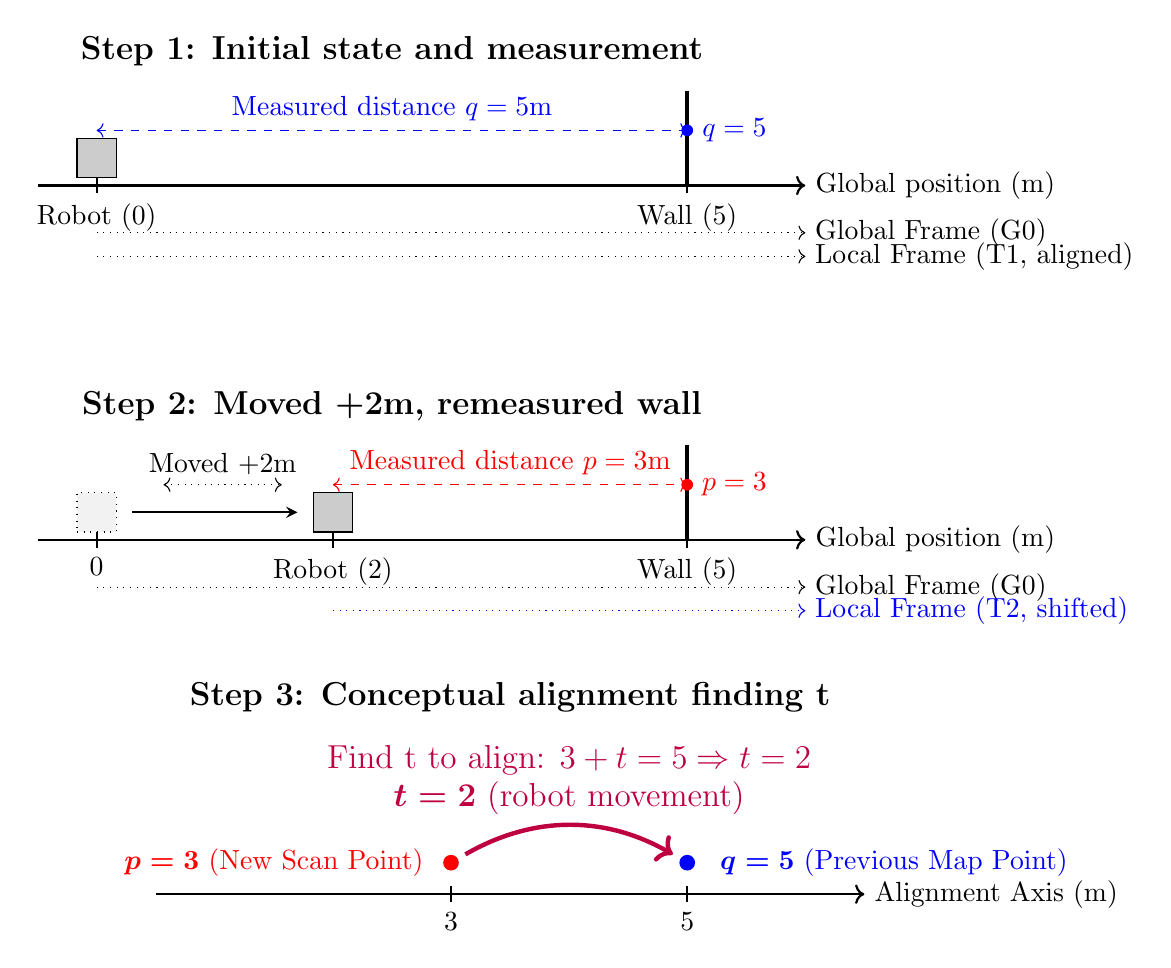
\begin{tikzpicture}[x=1.5cm]

  % ==========================================
  % SECTION 1: Initial state and measurement
  % ==========================================
  \begin{scope}[yshift=0cm]
    % Axis
    \draw[thick, ->] (-0.5,0) -- (6,0) node[right] {Global position (m)};
    \draw[thick] (0,0.1) -- (0,-0.1) node[below] {Robot (0)};
    \draw[thick] (5,0.1) -- (5,-0.1) node[below] {Wall (5)};
    \draw[->, dotted] (0,-0.6) -- (6,-0.6) node[right] {Global Frame (G0)};
    \draw[->, dotted, thin] (0, -0.9) -- (6, -0.9) node[right] {Local Frame (T1, aligned)};

    % Robot (visual representation)
    \node[draw, rectangle, minimum height=0.5cm, minimum width=0.5cm, fill=black!20] at (0,0.35) {};

    % Wall (visual representation)
    \draw[ultra thick] (5,0) -- (5,1.2);

    % Measurement (visual distance and scan point)
    \draw[<->, dashed, color=blue] (0,0.7) -- (5,0.7) node[midway, above, color=blue] {Measured distance $q=5$m};
    \node[circle, fill=blue, inner sep=1.5pt] at (5,0.7) {};
    \node[color=blue] at (5.4,0.7) {\color{blue} $q=5$};

    % Title
    \node[font=\large\bfseries] at (2.5,1.7) {Step 1: Initial state and measurement};
  \end{scope}

  % ==========================================
  % SECTION 2: After movement
  % ==========================================
  \begin{scope}[yshift=-4.5cm]
    % Axis
    \draw[thick, ->] (-0.5,0) -- (6,0) node[right] {Global position (m)};
    \draw[thick] (0,0.1) -- (0,-0.1) node[below] {0};
    \draw[thick] (2,0.1) -- (2,-0.1) node[below] {Robot (2)};
    \draw[thick] (5,0.1) -- (5,-0.1) node[below] {Wall (5)};
    \draw[->, dotted] (0,-0.6) -- (6,-0.6) node[right] {Global Frame (G0)};
    \draw[->, dotted, thin, blue] (2, -0.9) -- (6, -0.9) node[right, blue] {Local Frame (T2, shifted)};

    % Robot (current position)
    \node[draw, rectangle, minimum height=0.5cm, minimum width=0.5cm, fill=black!20] at (2,0.35) {};

    % Wall
    \draw[ultra thick] (5,0) -- (5,1.2);

    % Measurement (visual distance and new scan point)
    \draw[<->, dashed, color=red] (2,0.7) -- (5,0.7) node[midway, above, color=red] {Measured distance $p=3$m};
    \node[circle, fill=red, inner sep=1.5pt] at (5,0.7) {};
    \node[color=red] at (5.4,0.7) {\color{red} $p=3$};

    % Movement visualization (previous robot indicated lightly, movement text)
    \node[draw, rectangle, minimum height=0.5cm, minimum width=0.5cm, fill=black!5, dotted] at (0,0.35) {};
    \draw[thick, ->, >=stealth] (0.3,0.35) -- (1.7,0.35);
    \draw[<->, dotted, thin, xshift=1.3cm] (-0.3,0.7) -- (0.7,0.7) node[midway, above] {Moved +2m}; 

    % Title
    \node[font=\large\bfseries] at (2.5,1.7) {Step 2: Moved +2m, remeasured wall};
  \end{scope}

  % ==========================================
  % SECTION 3: Conceptual alignment finding t
  % ==========================================
  \begin{scope}[yshift=-9cm]
    % Axis (Alignment view)
    \draw[thick, ->] (0.5,0) -- (6.5,0) node[right] {Alignment Axis (m)};
    \draw[thick] (3,0.1) -- (3,-0.1) node[below] {3};
    \draw[thick] (5,0.1) -- (5,-0.1) node[below] {5};

    % Scan points
    \node[circle, fill=red, inner sep=2pt] (p) at (3,0.4) {};
    \node[circle, fill=blue, inner sep=2pt] (q) at (5,0.4) {};
    \node[color=red, font=\boldmath] at (1.5, 0.4) {\color{red} $p=3$ (New Scan Point)};
    \node[color=blue, font=\boldmath] at (6.75, 0.4) {\color{blue} $q=5$ (Previous Map Point)};

    % Alignment Arrow (shift p to q)
    \draw[ultra thick, ->, color=purple, shorten >=3pt, shorten <=3pt] (p) to[bend left=30] node[midway, above, color=purple, font=\boldmath] {\large $t=2$ (robot movement)} (q);

    % Annotation text
    \node[font=\large, color=purple] at (4,1.7) {\color{purple} Find t to align: $3 + t = 5 \Rightarrow t = 2$};

    % Title
    \node[font=\large\bfseries] at (3.5,2.5) {Step 3: Conceptual alignment finding t};
  \end{scope}

\end{tikzpicture}

\end{document}